% Options for packages loaded elsewhere
\PassOptionsToPackage{unicode}{hyperref}
\PassOptionsToPackage{hyphens}{url}
\PassOptionsToPackage{dvipsnames,svgnames,x11names}{xcolor}
%
\documentclass[
  10pt,
]{article}

\usepackage{amsmath,amssymb}
\usepackage{iftex}
\ifPDFTeX
  \usepackage[T1]{fontenc}
  \usepackage[utf8]{inputenc}
  \usepackage{textcomp} % provide euro and other symbols
\else % if luatex or xetex
  \usepackage{unicode-math}
  \defaultfontfeatures{Scale=MatchLowercase}
  \defaultfontfeatures[\rmfamily]{Ligatures=TeX,Scale=1}
\fi
\usepackage{lmodern}
\ifPDFTeX\else  
    % xetex/luatex font selection
\fi
% Use upquote if available, for straight quotes in verbatim environments
\IfFileExists{upquote.sty}{\usepackage{upquote}}{}
\IfFileExists{microtype.sty}{% use microtype if available
  \usepackage[]{microtype}
  \UseMicrotypeSet[protrusion]{basicmath} % disable protrusion for tt fonts
}{}
\makeatletter
\@ifundefined{KOMAClassName}{% if non-KOMA class
  \IfFileExists{parskip.sty}{%
    \usepackage{parskip}
  }{% else
    \setlength{\parindent}{0pt}
    \setlength{\parskip}{6pt plus 2pt minus 1pt}}
}{% if KOMA class
  \KOMAoptions{parskip=half}}
\makeatother
\usepackage{xcolor}
\setlength{\emergencystretch}{3em} % prevent overfull lines
\setcounter{secnumdepth}{-\maxdimen} % remove section numbering
% Make \paragraph and \subparagraph free-standing
\makeatletter
\ifx\paragraph\undefined\else
  \let\oldparagraph\paragraph
  \renewcommand{\paragraph}{
    \@ifstar
      \xxxParagraphStar
      \xxxParagraphNoStar
  }
  \newcommand{\xxxParagraphStar}[1]{\oldparagraph*{#1}\mbox{}}
  \newcommand{\xxxParagraphNoStar}[1]{\oldparagraph{#1}\mbox{}}
\fi
\ifx\subparagraph\undefined\else
  \let\oldsubparagraph\subparagraph
  \renewcommand{\subparagraph}{
    \@ifstar
      \xxxSubParagraphStar
      \xxxSubParagraphNoStar
  }
  \newcommand{\xxxSubParagraphStar}[1]{\oldsubparagraph*{#1}\mbox{}}
  \newcommand{\xxxSubParagraphNoStar}[1]{\oldsubparagraph{#1}\mbox{}}
\fi
\makeatother


\providecommand{\tightlist}{%
  \setlength{\itemsep}{0pt}\setlength{\parskip}{0pt}}\usepackage{longtable,booktabs,array}
\usepackage{calc} % for calculating minipage widths
% Correct order of tables after \paragraph or \subparagraph
\usepackage{etoolbox}
\makeatletter
\patchcmd\longtable{\par}{\if@noskipsec\mbox{}\fi\par}{}{}
\makeatother
% Allow footnotes in longtable head/foot
\IfFileExists{footnotehyper.sty}{\usepackage{footnotehyper}}{\usepackage{footnote}}
\makesavenoteenv{longtable}
\usepackage{graphicx}
\makeatletter
\def\maxwidth{\ifdim\Gin@nat@width>\linewidth\linewidth\else\Gin@nat@width\fi}
\def\maxheight{\ifdim\Gin@nat@height>\textheight\textheight\else\Gin@nat@height\fi}
\makeatother
% Scale images if necessary, so that they will not overflow the page
% margins by default, and it is still possible to overwrite the defaults
% using explicit options in \includegraphics[width, height, ...]{}
\setkeys{Gin}{width=\maxwidth,height=\maxheight,keepaspectratio}
% Set default figure placement to htbp
\makeatletter
\def\fps@figure{htbp}
\makeatother

\usepackage[margin=1in, top=0.6in]{geometry}
\usepackage{titlesec}
\titlespacing*{\title}{0pt}{0pt}{20pt}
\makeatletter
\@ifpackageloaded{caption}{}{\usepackage{caption}}
\AtBeginDocument{%
\ifdefined\contentsname
  \renewcommand*\contentsname{Table of contents}
\else
  \newcommand\contentsname{Table of contents}
\fi
\ifdefined\listfigurename
  \renewcommand*\listfigurename{List of Figures}
\else
  \newcommand\listfigurename{List of Figures}
\fi
\ifdefined\listtablename
  \renewcommand*\listtablename{List of Tables}
\else
  \newcommand\listtablename{List of Tables}
\fi
\ifdefined\figurename
  \renewcommand*\figurename{Figure}
\else
  \newcommand\figurename{Figure}
\fi
\ifdefined\tablename
  \renewcommand*\tablename{Table}
\else
  \newcommand\tablename{Table}
\fi
}
\@ifpackageloaded{float}{}{\usepackage{float}}
\floatstyle{ruled}
\@ifundefined{c@chapter}{\newfloat{codelisting}{h}{lop}}{\newfloat{codelisting}{h}{lop}[chapter]}
\floatname{codelisting}{Listing}
\newcommand*\listoflistings{\listof{codelisting}{List of Listings}}
\makeatother
\makeatletter
\makeatother
\makeatletter
\@ifpackageloaded{caption}{}{\usepackage{caption}}
\@ifpackageloaded{subcaption}{}{\usepackage{subcaption}}
\makeatother

\ifLuaTeX
  \usepackage{selnolig}  % disable illegal ligatures
\fi
\usepackage{bookmark}

\IfFileExists{xurl.sty}{\usepackage{xurl}}{} % add URL line breaks if available
\urlstyle{same} % disable monospaced font for URLs
\hypersetup{
  pdftitle={PPHA:30538 Final Project Writeup},
  pdfauthor={Cristian Bancayan, Claudia Felipe \& Sol Rivas Lopes},
  colorlinks=true,
  linkcolor={blue},
  filecolor={Maroon},
  citecolor={Blue},
  urlcolor={Blue},
  pdfcreator={LaTeX via pandoc}}


\title{\large PPHA:30538 Final Project Writeup}
\author{\normalsize Cristian Bancayan, Claudia Felipe \& Sol Rivas
Lopes}
\date{}

\begin{document}
\maketitle


\subsection{Motivation}\label{motivation}

Since the 1990s, Conditional Cash Transfers (CCTs) have been a key
anti-poverty program in Latin America and other developing regions.
These programs provide income subsidies to poor families, tied to their
children's school enrollment. While their success in boosting enrollment
and reducing poverty is well-documented, less research explores their
differing impacts on urban and rural areas. CCTs address income-driven
school withdrawals, common in both settings. However, they may not solve
low enrollment caused by limited school access, a problem more frequent
in rural areas with poor infrastructure.

Motivated by such discrepancies, this research project aims to
understand whether there is evidence of differential long-term impacts
of CCTs in education and quality of life outcomes in rural and urban
areas.

\begin{figure}[H]

{\centering 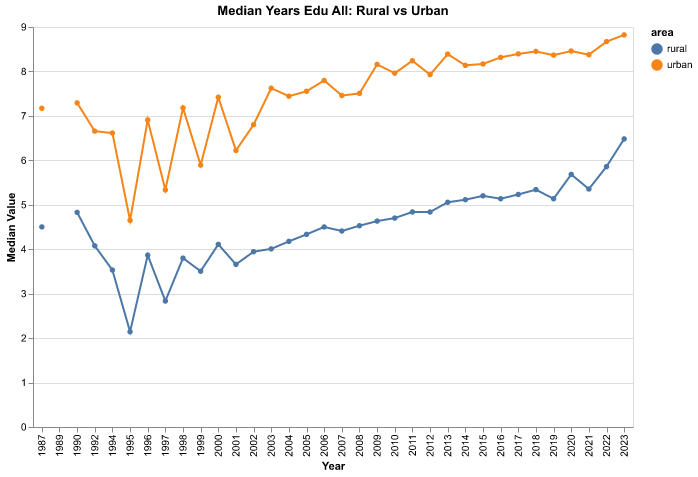
\includegraphics[width=0.4\textwidth,height=\textheight]{Graphs/years_edu_all.png}

}

\caption{The figure shows the aggregated median years of education in
Brazil, Chile, Mexico, Paraguay, and Peru. While there is a general
upward trend, urban populations have, on average, two more years of
education than rural populations. This pattern is consistent across all
countries, with disaggregated visualizations available in the Shiny
dashboard.}

\end{figure}%

\subsection{Data Source and Approach}\label{data-source-and-approach}

This project used data compiled by the Center for Distributive, Labor
and Social Studies (CEDLAS), from the National University of La Plata in
Argentina, in partnership with the World Bank. We retrieved datasets
about education, infrastrcutre, and housing, publicly available on their
\href{https://www.cedlas.econo.unlp.edu.ar/wp/en/estadisticas/sedlac/estadisticas/}{website}.

The cleaning process for the (\href{./cleaning_education.qmd}{education}
and \href{./cleaning_infraestructure.qmd}{infrastructure data}) selected
information depending on the survey methodologies for each country.
Then, for the analysis, we narrowed the datasets to include only the
target countries and variables of interest. Brazil, Chile, Mexico,
Paraguay, and Peru were chosen because they had both (a) implemented a
CCT program and (b) available rural and urban disaggregated data.
Variables were refined to focus only on relevant outcomes. We considered
years of education to gauge urban and rural disparities broadly.
However, we focused on school enrollment for 6- to 12-year-olds and 13-
to 17-year-olds to better capture immediate impacts of CCTs.

To explore outcomes beyond education, we examined changes to the quality
of life before and after CCT implementation. Because health, mental
health and labor force participation have been widely studied, we opted
to delve into the quality of dwellings. This addresses a gap in the
literature and considers that dwelling quality is less influenced by
systemic differences across countries. While health outcomes will vary
according to a country's public health and healthcare strucutre, a safe,
well-built house is likely to be consistent across all countires.
Furthermore, home improvement is an area where individuals have
significant autonomy and often allocate surplus income.

After cleaning and merging the data,
\href{./final_project_initial_analysis.qmd}{we created clear and
informative plots to visualize the data effectively}. We then conducted
simple regressions, correlation analyses, and t-tests to determine
whether the observed differences in the data were statistically
significant.

Given time limitations, the project did not aim to establish causal
relationships. All findings are based on descriptive and correlational
analyses, without robustness checks for causality. Nevertheless, the
insights gathered provide valuable descriptive information that can
inform future policy.

\subsection{Findings}\label{findings}

The main finding is that rural areas lead the increase in school
enrollment associated with the implementation of CCT programs. The
average percentage-point increase in rural school enrollment in the
periods after the implementation of a CCT program relative to periods
before exceeds that of urban areas across all countries.

Such improvements are particularly meaningful for the 13- to 17-year-old
group, suggesting that CCTs played a key role in keeping teenagers in
school. This indicates that the subsidies likely offset or outweigh the
immediate income benefits of enterging the workforce before school
completion. Furthermore, these improvements highlight that interruptions
in education are primarily driven by the need to supplement family
income.

\begin{figure}

\begin{minipage}{0.50\linewidth}
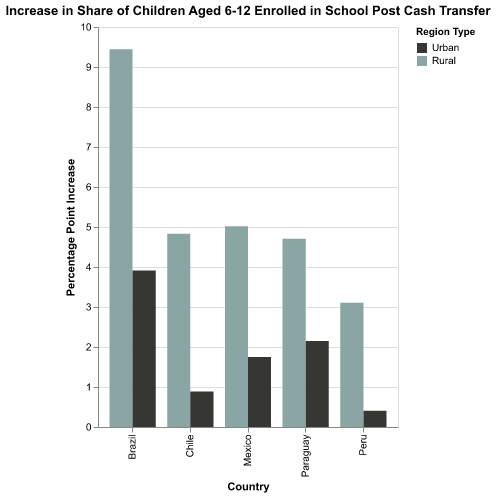
\includegraphics{Graphs/change_enrollment6_12yo.png}\end{minipage}%
%
\begin{minipage}{0.50\linewidth}
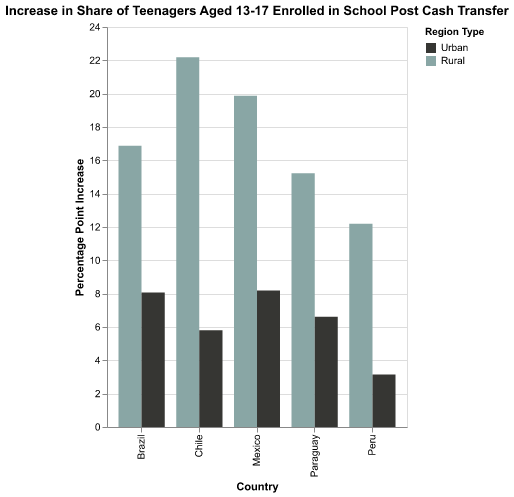
\includegraphics{Graphs/change_enrollment13_17yo.png}\end{minipage}%

\caption{\label{fig-combined}Figures 2a and 2b depict the average
percentage point increase in school enrollment following the
implementation of a CCT program in a given country, for 6- to
12-year-olds and 13- to 17-year-olds, respectively. Rural areas across
all countries consistently exhibit greater enrollment increases compared
to urban areas.}

\end{figure}%

We also explored how higher enrollment rates could translate into better
homes. Running a simple correlation, we found that in Brazil, Chile, and
Mexico, years of education and dwelling quality are highly inversely
correlated, with coefficients exceeding 0.9. In Paraguay, the
correlation is initially low, but after dropping two outliers, the same
linear relationship holds. Peru is the only country where these two
measures appear to be uncorrelated. These findings therefore suggest
that CCT programs indirectly and negatively might affect the share of
rural populations living in poor dwellings.

\begin{figure}[H]

{\centering 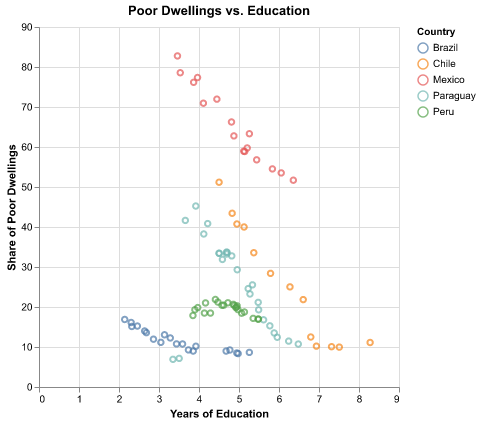
\includegraphics[width=0.4\textwidth,height=\textheight]{Graphs/corr_edu_dwelling.png}

}

\caption{The figure shows the correlation between years of education and
the average share of the population living in poor dwellings in rural
areas, disaggregated by country.}

\end{figure}%

This intuition is confirmed by visualizing how the share of poor
dwellings decreases after the implementation of CCT programs in each of
those 4 countries, even when effects are not immediate. A more
sophisticated identification strategy, such as a differences in
differences design, is needed to explore causality without confounding
factors. Still, these preliminary graphs are an optimistic start for
future research on the topic.

\begin{figure}

\begin{minipage}{0.50\linewidth}
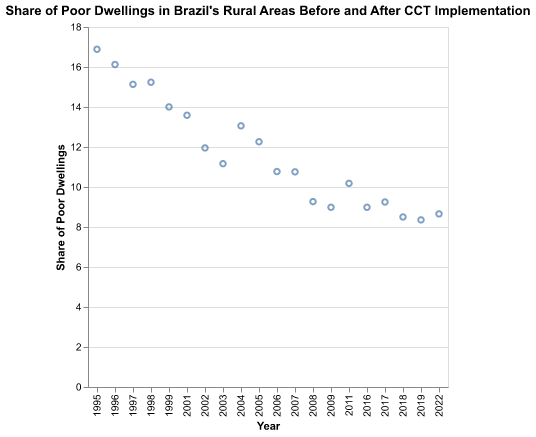
\includegraphics{Graphs/dwelling_Brazil.png}\end{minipage}%
%
\begin{minipage}{0.50\linewidth}
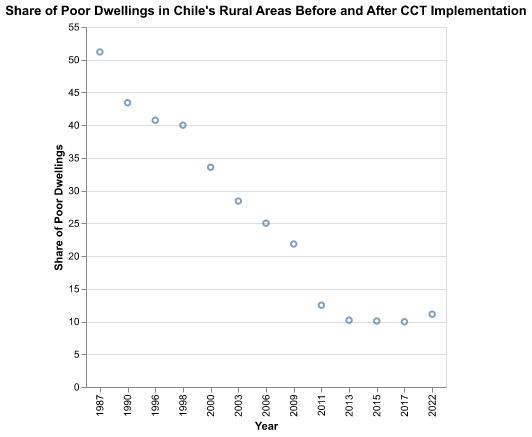
\includegraphics{Graphs/dwelling_Chile.png}\end{minipage}%

\caption{\label{fig-combined}Figures 4a and 4b shows the evolution of
the share poor dwellings after and before CCT implementation in Brazil
and Chile.}

\end{figure}%

For additional plots and comparisons, a \href{./shiny-app/app.py}{Shiny
dashboard} allows the user to allows explore trends for the outcomes
preivously mentioned across the five different countries analyzed.

\subsection{Policy Implications}\label{policy-implications}

Unlike our initial expectation, CCTs played a key role in increasing
enrollment rates, especially in rural areas. The long-term benefits go
beyond educational and financial gains, and could also possibly extend
to housing quality, although further research is needed in this respect.

Despite remaining disparities indicating a need for targeted
infrastrcure and education policies to better serve rural populations,
these findings reinforce the success of CCT programs as a transformative
force in breaking the cycle of poverty across both urban and rural
landscapes.




\end{document}
